\section{Evaluation}\label{sec:eval}

\subsection{Analysis of results}

As a result of our project, we managed to implement an ANN that uses deep reinforcement learning to learn playing the game Flappy Bird. We used a technique called "Double Deep Q Learning" to go beyond what we learned during the course. Apart form the mere fact that the network learned to play the game, we also gained some insights which we regard as the true learning success of this paper and we will present in the following.
\par
First, by building the environment ourselves, we learned how big of a role the environment and by that the possible inputs into a network play. At the beginning, we naively created our environment and thought that from that moment on, the task would only lie in finding the neural network architecture to work. But during the course of the project, we realized that tweaks to the environment can have a far greater influence on the networks learning behaviour. A prime example is how we implemented the reward: Our first version of the program gave the reward 1 if the bird passed a pipe, -1 if it hit a pipe or left the playing field and 0 for every other state. That led to a situation where the for almost all states, no reward could be gained. No matter how we tweaked our network, it did not learn. Only by changing the reward function into its current state, that the ANN receives positive reward if it is on the same height as the gap between the pipes, we could solve the issue of not learning. Giving the reward a Gaussian shape with the maximum at the center of the gap further increased the learning ability of the network.
\par
We also learned a lot by using a more sophisticated learning algorithm in the form of our Double Deep Q-Learning algorithm. We already learned architectures that use multiple ANNs during our course (for instance using an encoder and decoder to generate images), but still it was an interesting learning how a combination of multiple ANNs can improve the overall learning performance.
\par
Both these insights led to the more general insight: The singular network itself is not as important in deep learning as we thought it to be. The number and size of layers influences learning, but a changing what surrounds the network can also have a very significant influence. 
\par
In the following, we will evaluate the network in greater (technical) detail.

\subsection{Training}

As shown in Figure~\ref{fig:training-plot}, during training the average reward, epsilon magnitude, score and steps per episode were monitored.  
Score denotes the sum of all obtained rewards within a episode.
Note that the number of episode does not include the necessary episodes to fill the replay memory.
Before the actual training (changing network weights) begins, 250000 training samples (also called experiences) must be stored in the replay memory.
After about 400 episodes, the average reward decreases. 
However, at 600 episodes the average reward increases again.
Score and steps per episode increases over the entire training episodes.
Overall, the decrease of the average reward is irrelevant due to the actual goal: The model shall live (no collision with a column) as long as possible.
In other words, the goal was to increase the steps per episode.

\begin{figure}[h]
    \centering
    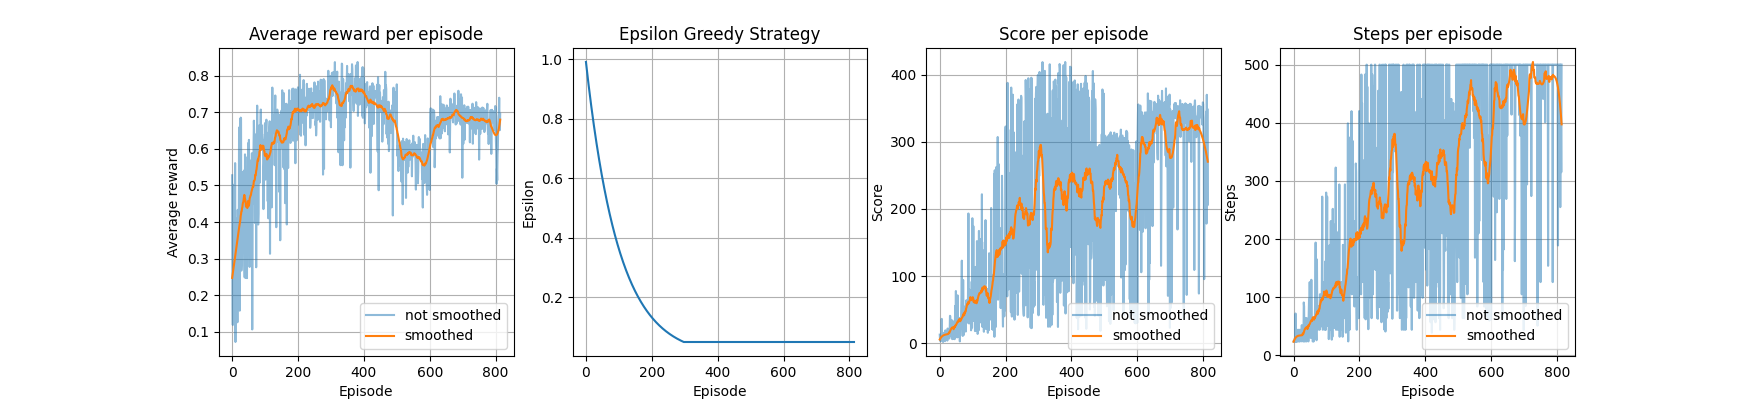
\includegraphics[width=\textwidth]{media/trainingPlot.png}
    \caption{Average reward, epsilon magnitude, score and steps per episode monitored during training.}
    \label{fig:training-plot}
\end{figure}

\subsection{Model Performance}

Figure~\ref{fig:performance-plot} presents the obtained rewards for 250 steps of the previously described model after tranining has finished. 
In average the model receives a reward of 0.8, which is rather high.
A collision with a column never occurred.
The downwards spikes of rewards followed with an immediate increase is caused by our reward calculation: Whenever the bird passes a column gap, the reward immediately is calculated for the next obstacle, which has a different height.
Since the model tries to maximize its reward by controlling the bird to be on the same height as the gap between the upcoming pipes, it vertically moves the bird towards the optimal position. 
As a consequence, the reward increases again.
\par
The small oscillations in reward are explained by the physical behaviour of the bird: It is always in the state of falling, and when the agent "flaps", it leaps upwards a certain height. 

\begin{figure}[h]
    \centering
    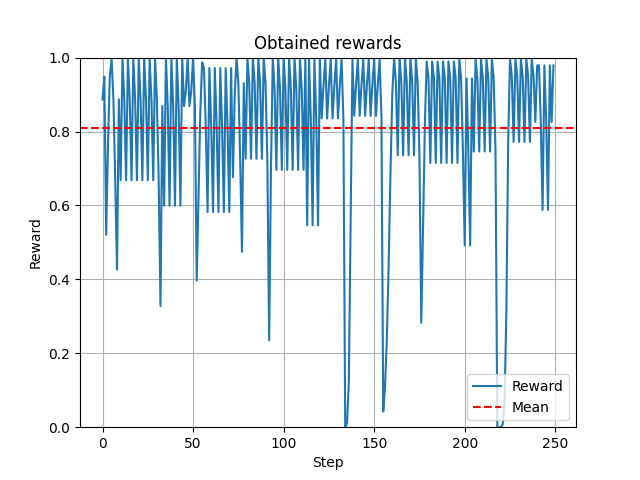
\includegraphics[width=\textwidth]{media/performancePlot.png}
    \caption{Running the model for 250 episodes.}
    \label{fig:performance-plot}
\end{figure}

\subsection{Comparison to related approaches}
As described in section \ref{sec:related}, there have been several related approaches, but only the one by Chen (\cite{chendeep}) has a similar focus as our project, as the others either use very different architectures (genetic algorithm) or have a different focus (as in \cite{performanceFB}. Hence, we will compare our project only to the former approach.
\par
One big difference between our approach and the one by Chen is the state. Chen passes the current frame, the current point in time and a parameter that dictates how many past frames have to be considered, while we only pass two times (current and past state) the 12 parameters as shown in listing \ref{listing:get-state}. Because of that, the network structure also differs: In order to process pixel-wise information, Chen uses convolutional layers which we do not need.
\par
Apart from these differences, the learning itself is rather similar. Chen does use not use the exact same Double Deep Q-Learning algorithm we use, although as described in section "Stability" \cite[p. 3]{chendeep}, he also uses an additional target network. The result is the same as ours, namely that the network learns to play the game.